\title{Models in Science - Final Report}
\author{Ryan Spangler}
\date{\today}

\documentclass[12pt]{article}

\usepackage{commath}
\usepackage{graphicx}

\setcounter{secnumdepth}{0}

\begin{document}
\maketitle

\section{Introduction}

One of the great mysteries of existence is that of experience.  How do the various individual actions of the components of the brain give rise to something which is a whole?  Somehow the punctuated spikes of single neurons {\em in synchrony} produce an integrated effect, a discrimination of separate features fused into a coherent, perceivable whole.  This is the mystery of consciousness, one of the mysteries that continues to elude us despite generations of our greatest efforts to unravel it.  It is all the more remarkable of a mystery because it is what composes ourselves, what we call ourselves.  It is the very basis of our own existence, yet the one thing that is seemingly beyond comprehension.  It would not be surprising if it relied on as-of-yet undiscovered physics (as certainly there must be much of) or require a severe conceptual realignment.  Obviously, a worthy challenge.

Clearly, this paper does not hope to tackle such a massive task.  It does not solve consciousness.  Though that is the motivation possibly, we must begin with humble steps.  What do we know?  From everything that we can tell, consciousness is correlated to cells firing in synchrony.  That is, when a particular subject is thought about, there is a corresponding synchronous activity in a particular assembly of neurons in the cortex.  These neurons can be distributed all throughout the brain, distance does not seem to be a deterrent to synchronization.  

One of the neural systems we know quite a bit about is the primary visual cortex, the initial gateway of direct visual information into the cortex, and there are some findings that reveal potential mechanisms for perception based on synchronization between populations of coordinating neural groups.  Some of these findings are nicely summarized by \cite{Sompolinsky}.  His subject is the orientation of bars that span a receptive field.  A receptive field he defines to be a set of neurons that discriminate different features of the same spatial area.  These receptive regions are spatially vaguely defined, but are mostly circular and include much overlap with neighboring regions.  Within a receptive field the neurons each respond to a different stimulus.  One responds to horizontal bars say, and others vertical ones, with a spectrum of various angles in between.  Some code for red, some for green.  Some are responsive to motion in one direction, some motion in another (motion alone can be decomposed into direction, speed, rotation or expansion/contraction).  All of these neurons belonging to a common receptive field are clustered together, each firing fairly specifically to a single modality and a single flavor of that modality, but interacting with each other through synaptic coupling.  If there is a vertical bar that is green for example, the neurons that fire when there is only a vertical bar will synchronize with the neurons that fire when in response to green, and each of these will activate inhibitory neurons that inhibit their complements.   This synchrony between mutually activated neurons is characteristic of activity within a receptive field.  

In addition to this action {\em within} a receptive field, there is also action {\em between} receptive fields.  This takes the character of synchronization between neurons which discriminate the same feature, but in neighboring receptive fields.  If the same vertical bar is detected in the neighboring field both vertical bar neurons will synchronize.  If the bar is broken, each vertical bar neuron will fire, but they may not synchronize.  This is accomplished through a system of weak coupling between them, whereas the coupling between neurons within a field are strongly coupled.  

All of this points to the functional role of synchronization in neural and cortical bases of perception.  Now that we know that synchronization is an important mechanism in the generation of experience, this leads to the question: how can synchronization be modeled?

\section{Models of Synchronization}

One of the most successful models of general mathematical synchronization is the Kuramoto model \cite{Acebrón} \cite{Ermentrout}.  The $N$ elements in the Kuramoto model are simple phase oscillators with a single phase variable $\theta$ and a preferred frequency $\omega$.  In addition, there is a connection matrix $K$ whose elements $K_{ij}$ express the strength of the coupling between the $i$th element to the $j$th element.  The equation as a whole is given by a differential equation for a given element $i$:

$$ \od{\theta_i}{t}=\omega_i+\sum\limits_{j=1}^N K_{ij}\sin(\theta_j-\theta_i)$$

where $i=1,...,N$.  So basically, this equation is a sum over the sine of all of the differences between a particular element and all of the other elements, scaled by the connection matrix.  The sine plays the functional role of emphasizing the differences between the phases.  The more different are the phases of each of the oscillators to the one in question, the more that element's phase will be adjusted.  If all of the elements happen to be in the same phase then the summing term would vanish and we would be left with the $\omega_i$, which is the element's natural frequency.  Left entirely to its own devices, the phase $\theta_i$ would be adjusted by its natural frequency $\omega_i$ each time step, and the phase would march merrily along a constant cycle.  

The Kuramoto model displays remarkable robustness to synchronization, and if no other factors come into play the elements will be swiftly phase-locked.  This model is straightforward to implement.  Here is the python code for a basic implementation of the Kuramoto model:

\begin{verbatim}
from pylab import *
tau = 2 * pi

class Kuramoto:
    def __init__(self, N, K=0.1, order=0.1):
        self.N = N
        self.K = K
        self.order = order
        self.scale = K / N
        self.reset()

    def reset(self):
        self.phase = random(self.N) * tau
        self.intrinsic = random(self.N) * self.order
        self.spikes = zeros(self.N)
        self.phases = self.phase

    def deltax(self, x):
        differences = sum(sin(self.phase - self.phase[x]))
        return self.intrinsic[x] + self.scale * differences

    def delta(self):
        return array(map(lambda x: self.deltax(x), range(self.N)))

    def step(self):
        self.phase += self.delta()
        self.spikes = vstack([self.spikes, where(self.phase >= tau, 1, 0)])
        self.phase = where(self.phase >= tau, self.phase - tau, self.phase)
        self.phases = vstack([self.phases, self.phase])

    def run(self, steps):
        self.reset()
        for step in range(steps):
            self.step()
\end{verbatim}

To use this code it is necessary to have a working installation of python with pylab (python's open source incarnation of matlab), then for $N=50$ elements running for 100 time steps invoke:

\begin{verbatim}
    from kuramoto import *
    model = Kuramoto(50)
    model.run(100)
    plot(model.phases)
\end{verbatim}

This is a direct implementation of the above equations for the Kuramoto model.  N is the number of elements and K is a universal connection factor (all elements are coupled equally to one another).  The behavior is striking:

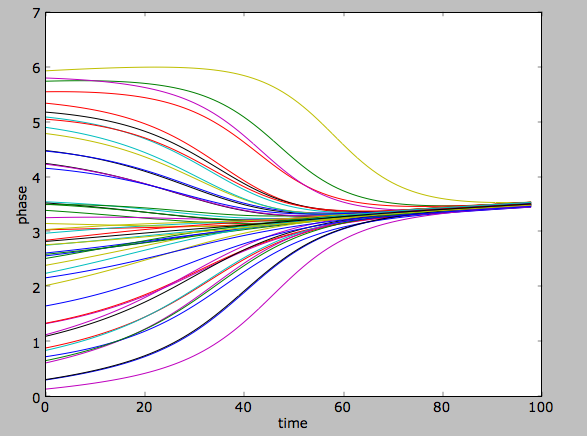
\includegraphics[scale=0.67]{kuramoto.png}

This is a plot of the phase of each element against time.  In the space of about 100 time steps the model was completely synchronized.  It can synchronize even more quickly if $K$ (the coupling) is raised.  

The Kuramoto model is impressive due to its strength of synchronization and its ultimate simplicity.  It is the perfect ingredient to more complex models, as is amply displayed in \cite{Acebrón}.  One of the intriguing applications of the Kuramoto model is Sompolinsky's work on the primary visual cortex \cite{Sompolinsky}.  This model attempts to capture the notion of interacting receptive fields discussed earlier.  Each neuron in the receptive field responds strongly to a single type of stimulus, ignoring all others.  All of the neurons within a receptive field code for a different stimulus, but this pattern of selectivity is repeated in each neighboring receptive field, so that there is in a sense a mirror image of the selectivities in each field.  The neurons which respond to a particular feature are weakly coupled between receptive fields.  

To model this Sompolinsky used a system based on the simplified Kuramoto model above, but with variable coupling strengths between neurons to represent the different receptive fields, and the notion of a stimulus and a tuning curve for each neuron representing its responsiveness to that stimulus.  Neurons within a cluster each respond to a different stimulus according to a tuning curve, and activated neurons are coupled strongly much like the Kuramoto model.  Neurons between clusters are coupled if they respond to the {\em same} stimulus.  

Another addition is that the firing of a neuron is taken to be a probabilistic event.  In concrete terms, the firing probability $P$ of a neuron is given by 

$$ P(\mathbf{r},t)=V(\mathbf{r})(1+\lambda\cos\Phi(\mathbf{r},t)) $$

where $\Phi(\mathbf{r},t)$ is the phase of neuron $\mathbf{r}$ at time $t$, $\lambda$ is the strength of the contribution of the other neurons to a particular neuron's phase, and $V(\mathbf{r})$ is that neuron's response to the stimulus presented:

$$ V(\mathbf{r})=V(\theta_0(\mathbf{r})-\theta(\mathbf{r})) $$

Here, $\theta_0(\mathbf{r})$ is an angle representation of the stimulus at neuron $\mathbf{r}$, and $\theta(\mathbf{r})$ is that neurons own preferred angle.  The tuning curve used is 

$$ V(\theta_0(\mathbf{r})-\theta(\mathbf{r}))=e^{-|\theta_0(\mathbf{r})-\theta(\mathbf{r})|/\sigma} $$

where $\sigma$ is some scaling constant.  This tuning curve is a sharp point at the selectivity orientation with exponential decay in both directions from that point.  The behavior of the phases $\Phi$ of the system is almost exactly that of the Kuramoto model (with an extra noise term $\eta$ added):

$$ \tau_0\od{\Phi(\mathbf{r},t)}{t}=\omega\tau_0+\eta(\mathbf{r},t)-\sum\limits_{r'}J(\mathbf{r},\mathbf{r}')\sin(\Phi(\mathbf{r},t)-\Phi(\mathbf{r'},t)) $$

The $\theta$s in the original model have been replaced with the phase function $\Phi$ and the noise term $\eta$ has been introduced, which is governed by white noise with variance proportional to $\tau_0$.  The function $J(\mathbf{r},\mathbf{r'})$ has replaced the matrix $K$ to represent the connectivity of the neurons to each other.  This function $J(\mathbf{r},\mathbf{r'})$ is crafted in such a way as to express the connectivity scheme as outlined above, namely, neurons are strongly coupled to other neurons in their same receptive field, and weakly coupled to neurons in other receptive fields that display the same selectivity as themselves.  

Officially, the form of $J(\mathbf{r},\mathbf{r'})$ is

$$ J(\mathbf{r},\mathbf{r'})=V(\mathbf{r})W(\mathbf{r},\mathbf{r'})V(\mathbf{r'}) $$

where the $V$ terms represent the activity of each neuron and $W$ is the connections matrix.  This means that if either of the neurons are inactive the effect will be greatly reduced.  For any real effect to take place, both neurons must be active at the same time.  

\section{Results}

The behavior of this model has important resemblances to the behavior of the primary visual cortex, and of course, huge differences.  The applicability of the model depends on what facet of the behavior of the system in question you are concerned with.  In this case, the model exhibited temporal coherence within clusters, and when the stimulus was similar between different clusters the synchronization extended across these clusters.  Also, synchronization occurred when the stimulus curved smoothly across receptive fields, showing that the system was able to interpolate across orientations that were near to each other and ``experience'' the entire curve in the form of synchronization and coherent activity, even from one end of the curve to the other where the orientations were no longer overlapping.  

The model is not the cortex of course.  These are phase variations and equations being run by a computer.  The simulation is useful in illuminating the dynamics of what would otherwise be a vaguely defined mechanism (the visual cortex).  The model itself can be used in a limited way in lieu of actual living cortical matter, and endless experiments can be run on it computationally without risking harm for living things actually using the cortical matter to experience the world for themselves.  It is specifically about synchronization for a particular stimulus (orientation of bars), so in a way relates only to that, but also the general method can be extended to any set of discriminations of interest. 

It is my hope that the study of synchronization will lead to a greater understanding of the nature and process of brain dynamics and ultimately consciousness.  The application of models, of whatever form, is the process of forging the necessary tools to understand and interact with the phenomenon itself, and is an indispensible part of any scientific inquiry.

\bibliographystyle{plain}
\bibliography{final}

\end{document} 
